\documentclass[10pt]{article}
\setlength{\parskip}{0.25\baselineskip}
\usepackage[margin=1in]{geometry} 
\usepackage{amsmath,amsthm,amssymb, graphicx, multicol, array}
\usepackage[font=small,labelfont=bf]{caption}

\newcommand{\supp}{{\text{supp}}} 
\newcommand{\bv}{{\text{BV}}}
\newcommand{\ac}{{\text{AC}}}

\newenvironment{problem}[2][]{\begin{trivlist}
\item[\hskip \labelsep {\bfseries #1}\hskip \labelsep {\bfseries #2.}]}{\end{trivlist}}

\begin{document}
 
\title{Homework \#1}
\author{Eric Tao\\
Math 123: Homework \#1}
\maketitle

\begin{problem}{Question 1}

Recall that for a matrix $A = (A_{ij})_{i,j=1}^n \in \mathbb{R}^{n\times n}$, and a vector $x = (x_1,...,x_n)^T \in \mathbb{R}^{n \times 1}$, matrix-vector multiplication is defined as $(Ax)_i = \Sigma_{k=1}^n A_{ik} x_k$. Prove that this operation is linear.

\end{problem}
\begin{proof}[Solution]

First, we wish to prove that for all $x,y \in \mathbb{R}^{n\times1}$, that $A(x+y) = Ax + Ay$. So, let $x,y$ be arbitrary vectors. Consider the i-th term of $A(x + y)$. By definition, this has form:

$$(A(x + y))_i = \Sigma_{k=1}^n A_{ik}(x_k+y_k) = \Sigma_{k=1}^n A_{ik}x_k + A_{ik}y_k = \Sigma_{k=1}^n A_{ik}x_k + \Sigma_{l=1}^n A_{il}y_l  = (Ax)_i + (Ay)_i $$

Since the choice of the i-th entry of $A(x+y)$ was arbitrary, this is true for every entry of $A(x+y)$. Thus, we have that $A(x+y) = Ax + Ay$.

Now, let $\alpha \in \mathbb{R}, x \in \mathbb{R}^{n\times1}$. We wish to show that $A(\alpha x) = \alpha Ax$. Again, we look at the $i-th$ term.

$$ (A(\alpha x))_i = \Sigma_{k=1}^n A_{ik} (\alpha x)_k =  \Sigma_{k=1}^n A_{ik} \alpha x_k = \alpha \Sigma_{k=1}^n A_{ik} x_k = \alpha(Ax)_i$$

Since, again, the choice of term was arbitrary, this is true for every term, and thus we may factor an $\alpha$ from each term; thus $A(\alpha x) = \alpha Ax$.

\end{proof}

\begin{problem}{Question 2}

Suppose $A \in \mathbb{R}^{n \times n}$ is a symmetric matrix. Denote $\mathbf{0} = (0,...,0) \in \mathbb{R}^n$ as the vector of all zeros. Prove that if $A$ has an eigenvalue of $0$, with associated eigenvector $x \not = \mathbf{0}$, then $A$ is not invertible. In particular, what can you say about the null space of $A$?

\end{problem}

\begin{proof}[Solution]

First of all, suppose $A$ has some eigenvector $u_i$ such that its eigenvalue $\lambda_i =0$. Because $A$ is symmetric, we may rewrite $A$ via singular value decomposition as:

$$ A = U^T \Lambda U$$

where $\Lambda$ is diagonal, composed of eigenvalues, and $U$ is orthogonal, composed of the eigenvectors. In particular, we consider the action of $U^T \Lambda U$ on $u_i$. Because $U$ is orthogonal, $U u_i$ is exactly a vector with 0 everywhere but the i-th entry, where we will denote this as $e_i$. $\Lambda e_i$ is exactly $\lambda_i e_i$, because $\Lambda$ is diagonal, this pulls out the i-th eigenvalue. And finally, $U^T \lambda_i e_i = \lambda_i u_i$ due to the shape of $U^T e_i$, pulling out the i-th column of $U^T$. But that's exactly the i-th row of $U$ that we started with. Thus, we have that:

$$A u_i = U^T \Lambda U u_i = \lambda_i u_i = 0 u_i = 0$$

Since $u_i \not = \mathbf{0}$ by hypothesis, we have found a non-0 vector such that $Au_i = 0$. Therefore, since the kernel of $A$ is non-trivial, $A$ is not invertible. Moreover, this implies that the nullspace of $A$ has dimension at least 1.

\end{proof}

\begin{problem}{Question 3}

Define the $l^2$ norm of $x \in \mathbb{R}^n$ to be

$$ \Vert x \Vert_2 = \sqrt{ \sum_{i=1}^n | x_i |^2}$$

Prove that $\Vert \cdot \Vert_2$ is a norm.

\end{problem}

\begin{proof}[Solution]

First, we wish to prove that for all $x \in \mathbb{R}^n$, that $\Vert x \Vert_2 \geq 0$. Since $x_i \in \mathbb{R}$, we have that $|x_i|^2 \geq 0$ for all $x_i$. Thus, $\sum_{i=1}^n |x_i|^2 \geq 0$, which implies that its square root is also non-negative.

Next, we want to prove that $\Vert x \Vert_2 \iff x = \mathbf{0}$. First, suppose $x = \mathbf{0}$. Then, $x_i = 0$ for all $i$. Thus, $\sum_{i=1}^n |x_i|^2 = \sum_{i=1}^n 0 = 0$, and the square root of 0 is certainly 0, so $\Vert \mathbf{0} \Vert_2 = 0$.

Now, suppose $\Vert x \Vert_2 = 0$. Then, squaring both sides, we must have that $\sum_{k=1}^n |x_i|^2 = 0$. But, due to the properties of the absolute value, since $|y| \geq 0$ for all $y \in \mathbb{R}$, for this to be true, $x_i = 0$ for all $i$. Thus, this implies $x = \mathbf{0}$ and we are done.

Now, let $\alpha \in \mathbb{R}, x \in \mathbb{R}^n$. We wish to show that $\Vert \alpha x \Vert_2 = |\alpha | \Vert x \Vert_2$. Well:

$$ \Vert \alpha x \Vert_2 =  \sqrt{ \sum_{i=1}^n | \alpha x_i |^2} = \sqrt{ \sum_{i=1}^n | \alpha|^2 | x_i |^2} = \sqrt{ |\alpha|^2 \sum_{i=1}^n | x_i |^2} = |\alpha|  \sqrt{ \sum_{i=1}^n |x_i |^2} = |\alpha| \Vert x \Vert_2 $$

Lastly, let $x,y \in \mathbb{R}^n$. We wish to show that $\Vert x + y \Vert_2 \leq \Vert x \Vert_2 + \Vert y \Vert_2$.

First, we recognize that the term underneath the square root can be identified as an inner product of two elements of $l^2$. That is, we may define $\langle x, y \rangle = \sum_{n=1}^\infty xy$. We notice that this satisfies the axioms of an inner product:

a) We have that $ 0 \leq \langle x, x \rangle$ because $x_i^2 \geq 0$ for all $x_i \in \{ x \}_{i=1}^\infty = x$, and $\langle x, x \rangle < \infty$ because $x \in l^2(\mathbb{R})$.

b) Because we work in the reals, we require symmetry, not conjugate symmetry, which comes from the commutativity of scalar multiplication.

c) Linearity in the first variable should be clear:

$$ \langle ax + by, z \rangle = \sum_{n=1}^\infty (ax_N + by_n)z_n = a \sum_{n=1}^\infty x_nz_n + b \sum_{n=1}^\infty y_nz_n = a \langle x,a \rangle  + b \langle y,z \rangle $$

d) $\langle x,x \rangle = 0 \iff x = 0$ should be clear. Clearly, if $x = 0$, then $\langle 0, 0 \rangle = \sum_{n=1}^\infty 0^2 = 0$. Now, if $\langle x, x \rangle = 0$, this implies that $\sum_{n=1}^\infty x_n^2 = 0$. But, for real numbers, $x_n^2 \geq 0$. Thus, for this to be true, $x_n = 0$ for all $n$, which implies $x$ is the sequence of all 0s.

So, we have an inner product on $l^2(\mathbb{R})$, and we notice that $\Vert x \Vert_2 = \sqrt{ \langle x,x \rangle}$.

Now, consider $\langle x + y, x+y \rangle$. By the linearity and commutativity of the real inner product, we have that

$$ \langle x + y , x + y \rangle = \langle x, x \rangle + 2 \langle x, y\rangle + \langle y,y \rangle $$

but, by Cauchy-Schwarz, we have that:

$$  \langle x + y , x + y \rangle = \langle x, x \rangle + 2 \langle x, y \rangle + \langle y,y \rangle \leq \langle x, x \rangle + 2 |\langle x, y\rangle| + \langle y,y \rangle \leq $$
$$ \langle x,x \rangle + \langle y,y\rangle + 2\sqrt{ \langle x,x\rangle \langle y,y \rangle} = \left(\sqrt{\langle x,x\rangle } + \sqrt{\langle y,y \rangle}\right)^2 $$

Taking the square root of both sides, which we can do because $\langle x +y, x+y \rangle,  \langle x,x \rangle,  \langle y,y\rangle \geq 0$, we find that:

$$ \sqrt{ \langle x + y , x + y \rangle} \leq \sqrt{\langle x,x\rangle } + \sqrt{\langle y,y \rangle}$$

But, by our original remark, this is exactly the statement that:

$$ \Vert x+y \Vert_2 \leq \Vert x \Vert_2 + \Vert y \Vert_2 $$
\end{proof}

\begin{problem}{Question 4}

Suppose $(x_1, y_1), (x_2,y_2),...,(x_n,y_n) \in \mathbb{R}^2$ are sampled from a line $y = \alpha x$, for some $\alpha \in \mathbb{R}$. Prove that the empirical covariance matrix has rank $1$.

\end{problem}

\begin{proof}[Solution]

First, for convenience, denote $\overline{x_i} = (x_i, y_i)$, that is, a matrix of dimension $1 \times 2$. Since these are sampled from a line, we may rewrite $\overline{x_i} = (x_i, \alpha x_i)$. We recall that to compute the empirical covariance matrix, we simply need to take:

$$ \frac{1}{n} \sum_{k=1}^n  \overline{x_i}^T \overline{x_i}$$

Ignoring the $\frac{1}{n}$ term, as it has no bearing on the rank of a matrix, fix a specific $i$. The product has form:

$$  \overline{x_i}^T \overline{x_i} = \begin{bmatrix} x_i \\ \alpha x_i \end{bmatrix} \begin{bmatrix} x_i  & \alpha x_i \end{bmatrix} = \begin{bmatrix} x_i^2 & \alpha x_i^2 \\ \alpha x_i^2 & \alpha^2 x_i^2 \end{bmatrix} $$

Then, putting this back into the sum, we have that:

$$ \sum_{k=1}^n  \overline{x_i}^T \overline{x_i} = \begin{bmatrix} \sum_{i} x_i^2 & \alpha \sum_i x_i^2 \\ \alpha\sum_i x_i^2 & \alpha^2 \sum_i x_i^2 \end{bmatrix} $$

where we use $\sum_i$ as shorthand for $\sum_{i=1}^n$. 

First, suppose $\alpha = 0$. Then, this matrix is exactly:

$$ \begin{bmatrix} \sum_i x_i^2 & 0 \\ 0 & 0 \end{bmatrix} $$

which, if we assume that at least one $x_i \not = 0$, has one 0 column vector and one non-0 column vector, which is rank 1.

Now, suppose $\alpha \not = 0$. Then, we see that, as column vectors, that $\alpha \begin{bmatrix}  \sum_{i} x_i^2 \\ \alpha \sum_i x_i^2  \end{bmatrix} = \begin{bmatrix} \alpha  \sum_i x_i^2 \\ \alpha^2 \sum_i x_i^2 \end{bmatrix}$. Therefore, this matrix is still rank 1, assuming that at least one $x_i \not = 0$.

Of course, if we happen to only sample the point $(0,0)$, our empirical covariance matrix will be identically 0 and have rank 0.


\end{proof}

\begin{problem}{Question 5}

In MATLAB, run 'HW1.m' to get the data X\_Circle, consisting of uniformly sampled points from the interior of a ball in $\mathbb{R}^2$, and X\_Ellipse, consisting of uniformly sampled points on the interior of an ellipse in $\mathbb{R}^2$.

(a) In MATLAB, compute the two principal components of X\_Circle from the definition in terms of the covariance matrix. Do they have geometric significance for this data?

(b) In MATLAB, compute the two principal components of X\_Ellipse from the definition in terms of the covariance matrix. Do they have geometric significance for this data?

\end{problem}

\begin{proof}[Solution]

(a)

Using the provided code, we compute the empirical covariance matrix by iterating over the data points, and summing up $2 \times 2$ mat rices that have the form $X^T X$, where $X = ( x , y)$, a row vector of $(x,y)$-coordinates of the circle. Then, the eigenvectors and values of the empirical covariance matrix were computed, and the principal components identified as the eigenvectors. An example of the output is shown below, where $v$ denotes the right eigenvectors, $w$ denotes left eigenvectors, and $d$ denotes the eigenvalues. 

\begin{center}
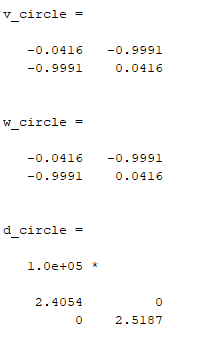
\includegraphics[,scale=0.5]{circle_data}
\captionof{figure}{}
\end{center}

We notice that the eigenvalues are approximately equal, within $10\%$ of each other. Further, if we run the program multiple times, we notice that although the exact components computed vary greatly, however, the two eigenvalues stay roughly equal. This implies that the exact eigenvectors are products of the sampling, and the geometric interpretation is that a circle has infinite rotational symmetries, and that any choice of eigenbasis to describe the data points largely is arbitrary, dependent on the randomness in the sampling.

(b)

In a similar fashion, we do the same procedure for the ellipse.

\begin{center}
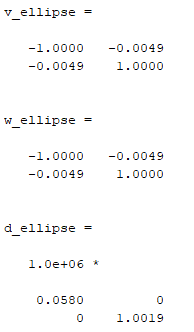
\includegraphics[,scale=0.5]{ellipse_data}
\captionof{figure}{}
\end{center}

We notice that in this case, there are two eigenvectors that distinguish themselves, one with larger eigenvalue. This relates to the shape of the ellipse, where we have two lines of reflection, along the major and minor axes, in this case, the x and y-axes. In this case, the geometric intuition should be that these represent that directions of maximum variance in our points, as the axes represent the largest distance two lines can take up within the ellipse - the major axis of course providing the direction of maximum variance.


\end{proof}

 

\end{document}